\section{Face validation}
The problem of face validation in our context is represented by determining whether the face detected in an image belongs to a live subject or it is on a printed photo, replayed video or 3D mask. Various methods to combat such attacks have been studied and they include: face motion analysis \cite{BharadwajDVS13},\cite{PanSWL07},\cite{TirunagariPWISH15} like eye blink, lip or head movement that is effective in combating printed photos attack, face 3D shape or depth analysis \cite{MarsicoNRD12}, \cite{LagorioTCFS13} which is useful in combating 2D attacks but may require additional device, face texture analysis \cite{MaattaHP11} which have computationally low costs and are fast but might encounter difficulties in generalizability. Our implementation of the face spoof detector is based on the work of Maatta et al. presented in \cite{MaattaHP11} where the proposed approached is based on the analysis of face texture using multi-scale local binary patterns (MLBP).
\subsection{Local Binary Patterns}
The LBP is a type of visual descriptor used for texture identification and classification. It is a particular case of the Texture Unit model described in 1990 in \cite{HeWang90}. The idea proposed by He\&Wang in \cite{HeWang90} was to compute the local texture for each pixel in an image based on a surrounding neighborhood of $3\times3$ pixels. The way to compute it was to compare the intensity of the central pixel $V_c$ with the intensity of each of the 8 neighbour pixels $V_{i=\overline{1,8}}$so resulting a corresponding texture unit TU with 8 elements calculated as this:
\begin{align}
	E_i = \begin{cases}
	0, & if\ V_i < V_c \\
	1, & if\ V_i = V_c \\
	2, & if\ V_i > V_c
	\end{cases}
\end{align}
The texture unit representation is then seen as a number in base 3 and transform in decimal base obtaining this way a number describing the local texture of a pixel.
A visual representation can be seen in figure 2.4
\begin{figure}[h]
	\begin{center}
		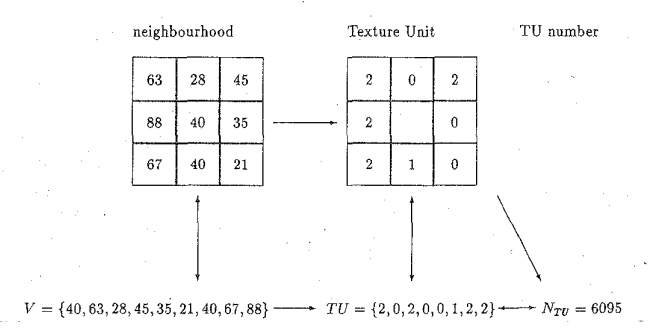
\includegraphics[width=15cm]{texture-unit-transform}
	\end{center}
	\caption[Visual representation of texture unit transform]{How \cite{HeWang90} presented the transformation of a pixel neighbourhood into a texture unit and a texture unit number}
\end{figure}

The reason why LBP is considered to be a particular case of texture unit is that it's function of computing the $E_i$ differs from the one proposed by He\&Wang in that the equality case is comprised in 